\documentclass{article}
% Change "article" to "report" to get rid of page number on title page
\usepackage{amsmath,amsfonts,amsthm,amssymb}
\usepackage{setspace}
\usepackage{Tabbing}
\usepackage{fancyhdr}
\usepackage{lastpage}
\usepackage{extramarks}
\usepackage{chngpage}
\usepackage{soul,color}
\usepackage{graphicx,float,wrapfig}
\usepackage{multicol}
\usepackage{cancel}




% In case you need to adjust margins:
\topmargin=-0.45in      %
\evensidemargin=0in     %
\oddsidemargin=0in      %
\textwidth=6.5in        %
\textheight=9.0in       %
\headsep=0.25in         %

% envit Specific Information
\newcommand{\envitTitle}{Geometr\'ia de la Antena de 3.5 m}
\newcommand{\envitDate}{2015}
\newcommand{\envitField}{Radioastronom\'ia}
\newcommand{\envitInstitution}{Universidad ECCI}
\newcommand{\envitAuthor}{G. Chaparro}
\newcommand{\envitAuthorName}{}

% Setup the header and footer
\pagestyle{fancy}                                                       %
\lhead{\envitAuthorName}                                                 %
\chead{\envitField\ |\envitAuthor |\ \envitInstitution |  \envitTitle}  %
%\rhead{\firstxmark}                                                     %
\rhead{}
\lfoot{\lastxmark}                                                      %
\cfoot{\envitDate}                                                                %
\rfoot{P\'agina\ \thepage\ de\ \pageref{LastPage}}                          %
\renewcommand\headrulewidth{0.4pt}                                      %
\renewcommand\footrulewidth{0.4pt}                                      %

% This is used to trace down (pin point) Items
% in latexing a document:
%\tracingall

%%%%%%%%%%%%%%%%%%%%%%%%%%%%%%%%%%%%%%%%%%%%%%%%%%%%%%%%%%%%%
% Some tools
\newcommand{\enterItemHeader}[1]{\nobreak\extramarks{#1}{#1 contin\'ua en la pr\'oxima p\'agina\ldots}\nobreak%
                                    \nobreak\extramarks{#1 (continued)}{#1 contin\'ua en la pr\'oxima p\'agina\ldots}\nobreak}%
\newcommand{\exitItemHeader}[1]{\nobreak\extramarks{#1 (contin\'ua)}{#1 contin\'ua en la pr\'oxima p\'agina\ldots}\nobreak%
                                   \nobreak\extramarks{#1}{}\nobreak}%

\newlength{\labelLength}
\newcommand{\labelBoxedItem}[2]
  {\settowidth{\labelLength}{#1}%
   \addtolength{\labelLength}{0.25in}%
   \changetext{}{-\labelLength}{}{}{}%
   \noindent\fbox{\begin{minipage}[c]{\columnwidth}#2\end{minipage}}%
   \marginpar{\fbox{#1}}%

   % We put the blank space above in order to make sure this
   % \marginpar gets correctly placed.
   \changetext{}{+\labelLength}{}{}{}}%

\setcounter{secnumdepth}{0}
\newcommand{\environmentItemName}{}%
\newcounter{environmentItemCounter}%
\newenvironment{environmentItem}[1][\'Item \arabic{environmentItemCounter}]%
  {\stepcounter{environmentItemCounter}%
   \renewcommand{\environmentItemName}{#1}%
   \section{\environmentItemName}%
   \enterItemHeader{\environmentItemName}}%
  {\exitItemHeader{\environmentItemName}}%

\newcommand{\boxedsubitem}[1]
  {\noindent\fbox{\begin{minipage}[c]{\columnwidth}#1\end{minipage}}}%

\newcommand{\ItemLBoxedItem}[1]
  {\labelBoxedItem{\environmentItemName}{#1}}

\newcommand{\envitSectionName}{}%
\newlength{\envitSectionLabelLength}{}%
\newenvironment{envitSection}[1]%
  {% We put this space here to make sure we're not connected to the above.
   % Otherwise the changetext can do funny things to the other margin

   \renewcommand{\envitSectionName}{#1}%
   \settowidth{\envitSectionLabelLength}{\envitSectionName}%
   \addtolength{\envitSectionLabelLength}{0.25in}%
   \changetext{}{-\envitSectionLabelLength}{}{}{}%
   \subsection{\envitSectionName}%
   \enterItemHeader{\environmentItemName\ [\envitSectionName]}}%
  {\enterItemHeader{\environmentItemName}%

   % We put the blank space above in order to make sure this margin
   % change doesn't happen too soon (otherwise \sectionBoxedItem's can
   % get ugly about their \marginpar placement.
   \changetext{}{+\envitSectionLabelLength}{}{}{}}%

\newcommand{\sectionBoxedItem}[1]
  {% We put this space here to make sure we're disconnected from the previous
   % passage

   \noindent\fbox{\begin{minipage}[c]{\columnwidth}#1\end{minipage}}%
   \enterItemHeader{\environmentItemName}\exitItemHeader{\environmentItemName}%
   \marginpar{\fbox{\envitSectionName}}%

   % We put the blank space above in order to make sure this
   % \marginpar gets correctly placed.
   }%

%%%%%%%%%%%%%%%%%%%%%%%%%%%%%%%%%%%%%%%%%%%%%%%%%%%%%%%%%%%%%


%%%%%%%%%%%%%%%%%%%%%%%%%%%%%%%%%%%%%%%%%%%%%%%%%%%%%%%%%%%%%
% Make title
\title{\vspace{2in}\textmd{\textbf{\envitField:\ \envitTitle}}\\\normalsize\vspace{0.1in}\small{\ on\ \envitDate}\\\vspace{0.1in}\large{\textit{\envitAuthor\ \envitInstitution}}\vspace{3in}}
\date{}
\author{\textbf{\envitAuthorName}}
%%%%%%%%%%%%%%%%%%%%%%%%%%%%%%%%%%%%%%%%%%%%%%%%%%%%%%%%%%%%%

\begin{document}
\begin{spacing}{1.1}
%\maketitle
%\newpage
% Uncomment the \tableofcontents and \newpage lines to get a Contents page
% Uncomment the \setcounter line as well if you do NOT want subsections
%       listed in Contents
%\setcounter{tocdepth}{1}
%\tableofcontents
%\newpage

% When Items are long, it may be desirable to put a \newpage or a
% \clearpage before each environmentItem environment

%\clearpage
\begin{center}
\LARGE{\textbf{\envitTitle}}\\
\end{center}
\normalsize



\begin{environmentItem}[Azimuth]
Puntos fijos: P1, P2
Distancia variable: $D_{34}$, $D_{23}$
\begin{center}
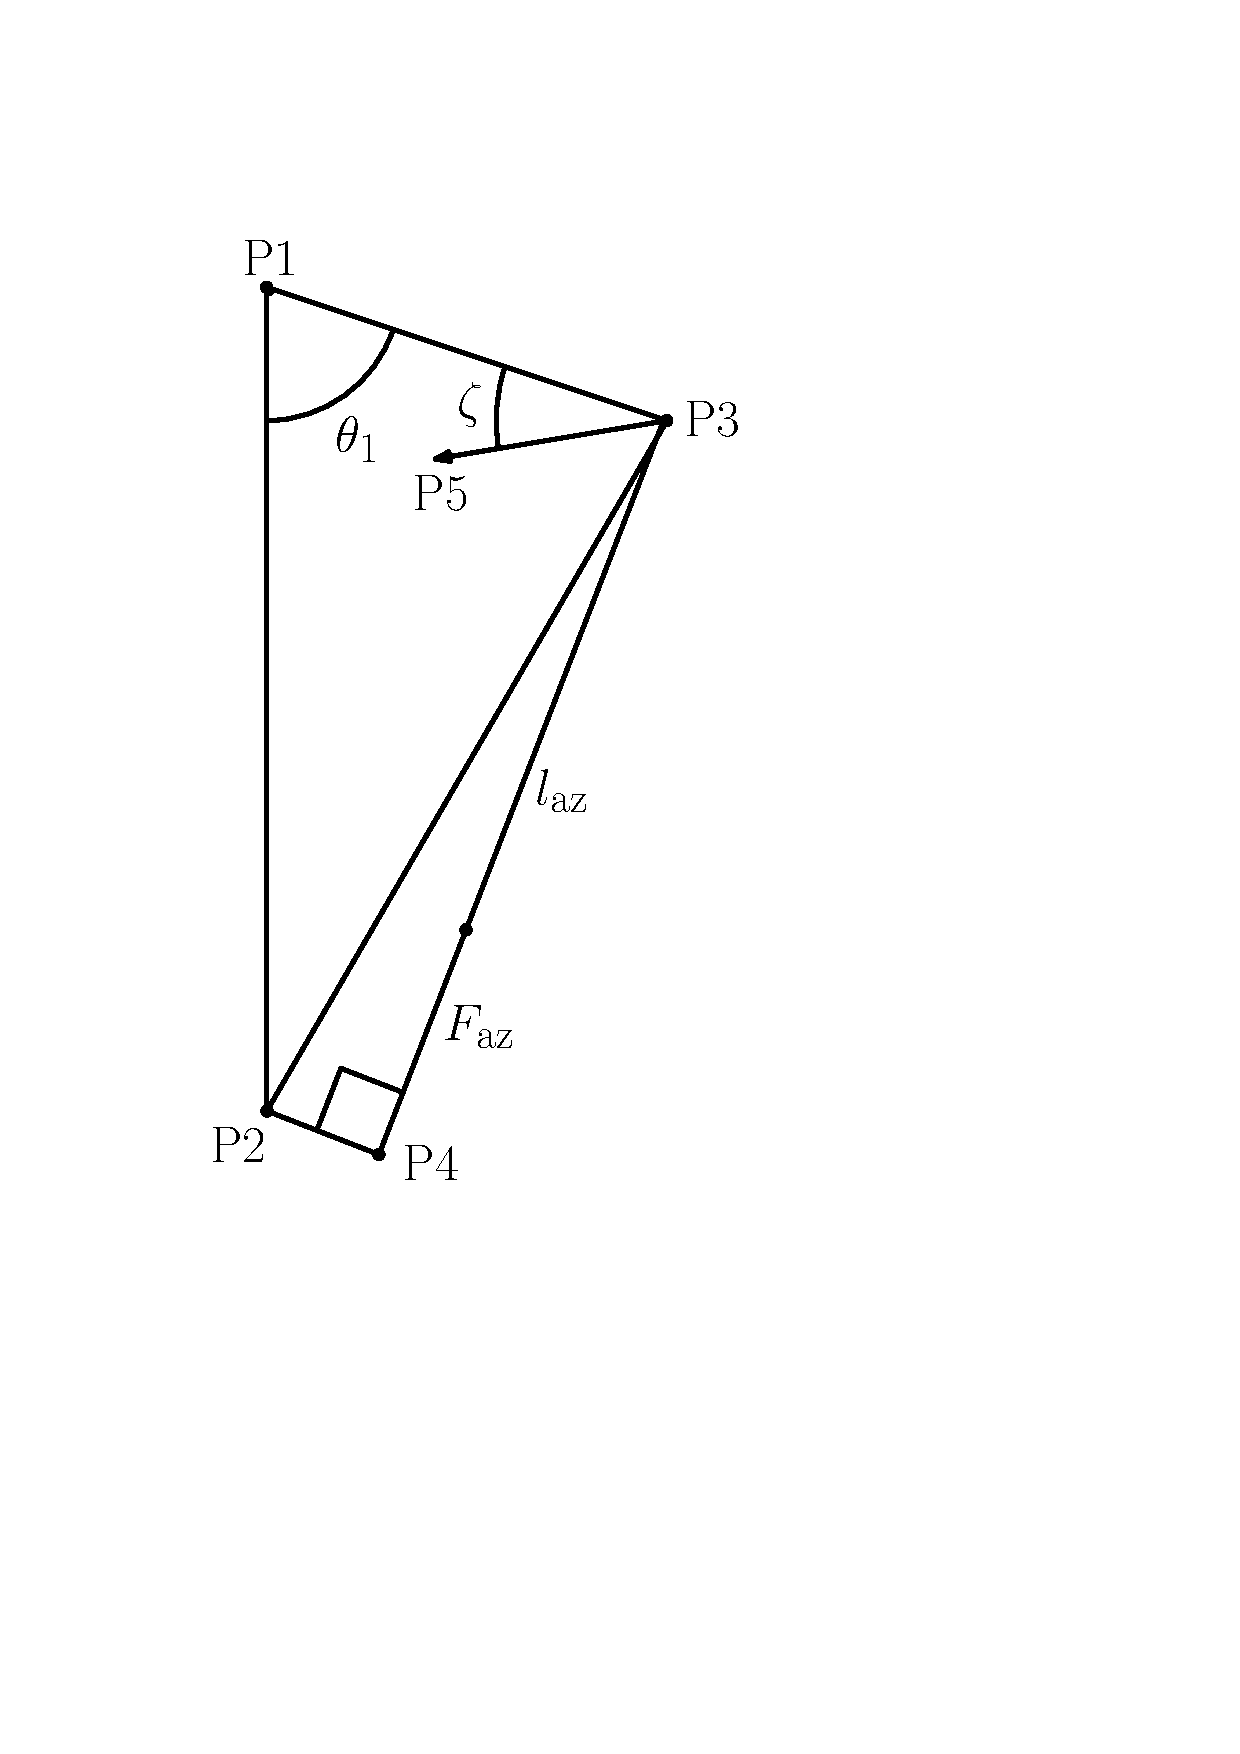
\includegraphics[scale=0.5]{azimuth}\\
\end{center}
\begin{itemize}
\item P1: Anclaje principal
\item P2: Anclaje motor
\item P3: Anclaje sinf\'in/Eje Antena
\item P4: Abrazadera sobre el motor
\item P5: Foco del telescopio
\item $F_\mathrm{az}$= Longitud fija del motor (housing) desde P4
\item $l_\mathrm{az}$= Longitud del sinf\'in
\end{itemize}

\boxedsubitem{
\[D_{23}^2=D_{12}^2+D_{13}^2-2D_{12}D_{13}\cos\theta_1\]
\[D_{34}=F_\mathrm{az}+l_\mathrm{az}\]
\[D_{23}^2=D_{24}^2+(F_\mathrm{az}+l_\mathrm{az})^2\]
\[\cos\theta_1=\frac{D_{12}^2+D_{13}^2-D_{24}^2-(F_\mathrm{az}+l_\mathrm{az})^2}{2D_{12}D_{13}}\]
\[\theta_1(l_\mathrm{az})=\cos^{-1}\left(\frac{D_{12}^2+D_{13}^2-D_{24}^2-(F_\mathrm{az}+l_\mathrm{az})^2}{2D_{12}D_{13}}\right)+\zeta\]

}
\end{environmentItem}

\begin{environmentItem}[Elevation]
Puntos fijos: P1, P2
Distancia variable: $D_{34}$, $D_{23}$
\begin{center}
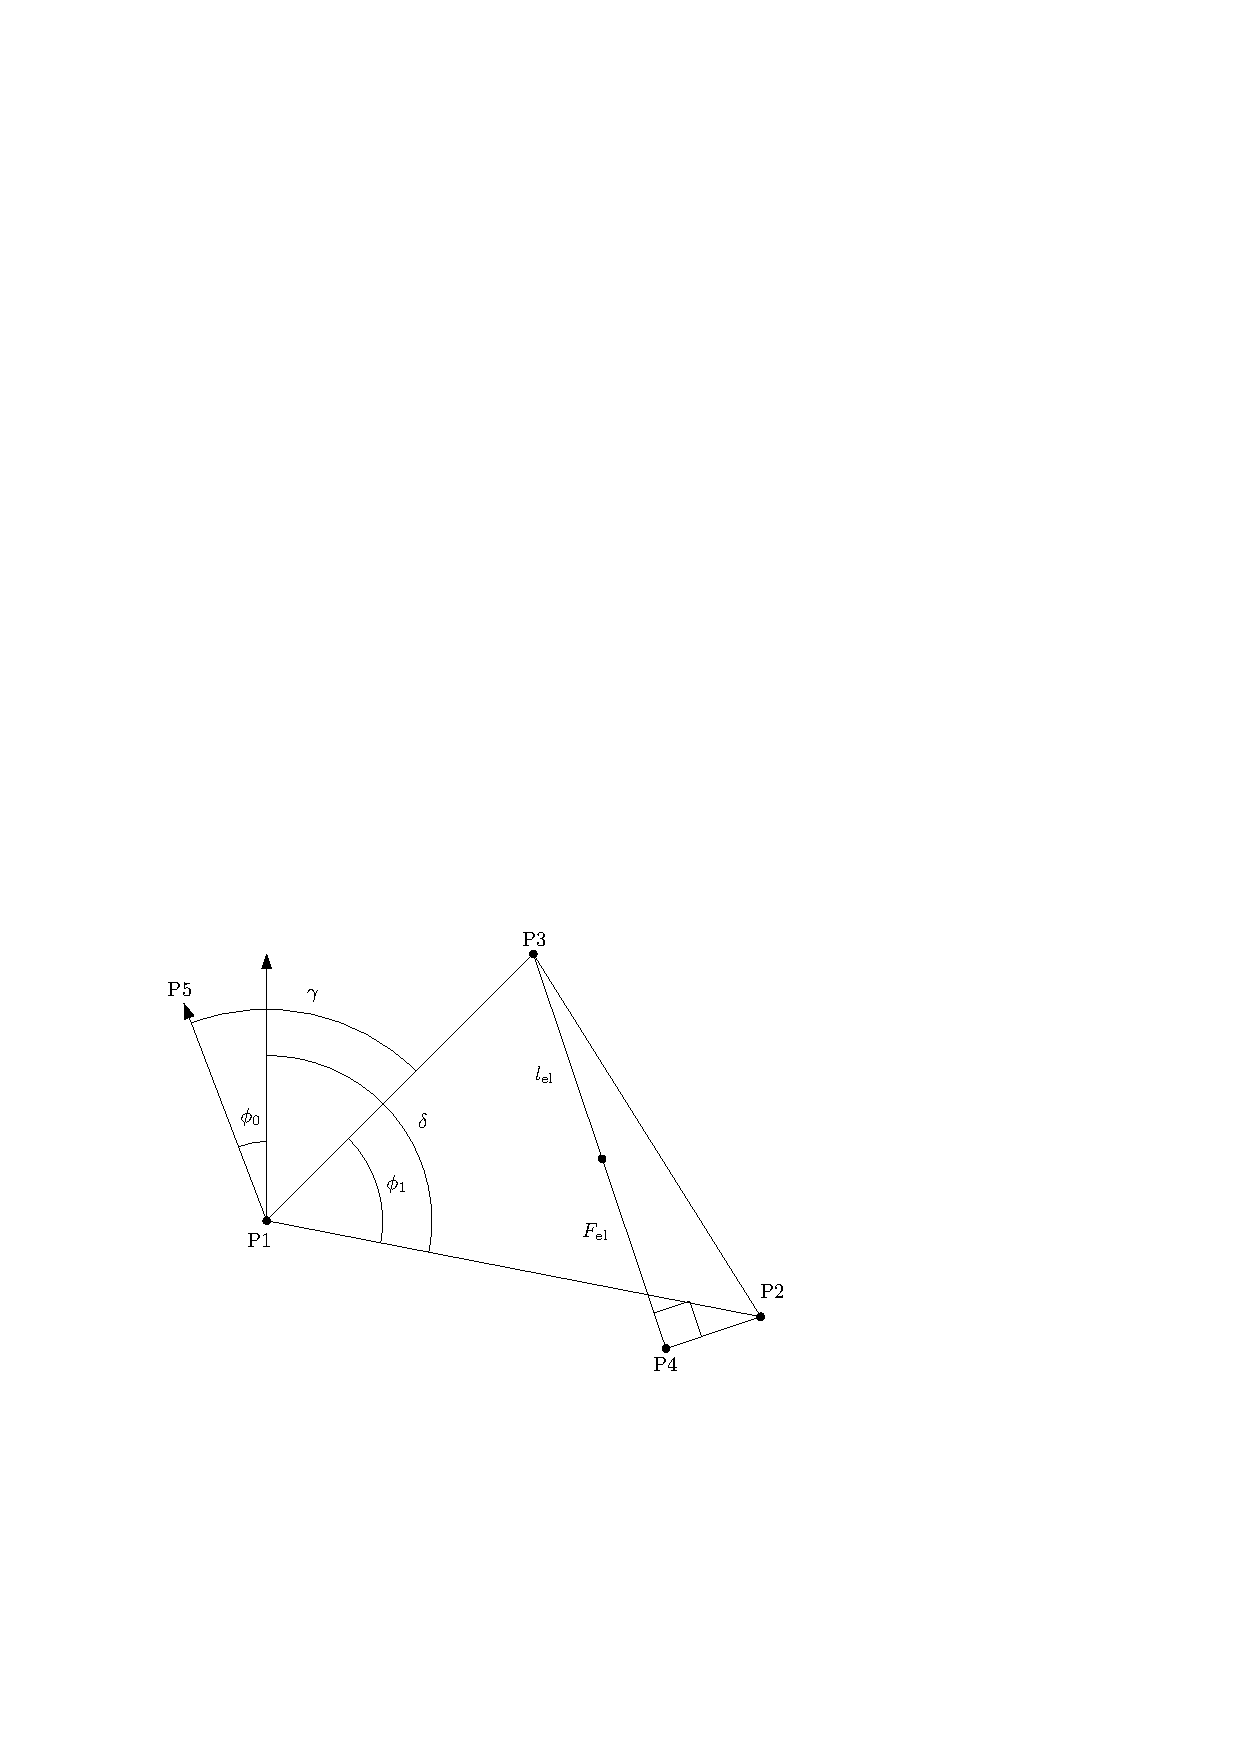
\includegraphics[scale=1.5]{elevation}\\
\end{center}
\begin{itemize}
\item P1: Anclaje principal
\item P2: Anclaje sinf\'in-Eje Plato
\item P3: Anclaje motor
\item P4: Abrazadera sobre el motor
\item P5: Foco del Telescopio
\item $F_\mathrm{el}$= Longitud fija del motor (housing) desde P4
\item $l_\mathrm{el}$= Longitud del sinf\'in
\end{itemize}

\boxedsubitem{
\[\phi_1+\gamma=\phi_0+\delta\]
\[\phi_0=\phi_1+\gamma-\delta\]
\[D_{23}^2=(F_\mathrm{el}+l_\mathrm{el})^2+D_{24}^2\]
\[D_{23}^2=D_{12}^2+D_{13}^2-2D_{12}D_{13}\cos\phi_1\]
\[\cos\phi_1=\frac{D_{12}^2+D_{13}^2-(F_\mathrm{el}+l_\mathrm{el})^2-D_{24}^2}{2D_{12}D_{13}}\]
\[\phi_0(l_\mathrm{el})=\cos^{-1}\left(\frac{D_{12}^2+D_{13}^2-(F_\mathrm{el}+l_\mathrm{el})^2-D_{24}^2}{2D_{12}D_{13}}\right)+\gamma-\delta\]
}
\end{environmentItem}


\end{spacing}
\end{document}

%%%%%%%%%%%%%%%%%%%%%%%%%%%%%%%%%%%%%%%%%%%%%%%%%%%%%%%%%%%%%

%----------------------------------------------------------------------%
% The following is copyright and licensing information for
% redistribution of this LaTeX source code; it also includes a liability
% statement. If this source code is not being redistributed to others,
% it may be omitted. It has no effect on the function of the above code.
%----------------------------------------------------------------------%
% Copyright (c) 2007, 2008, 2009, 2010, 2011 by Theodore P. Pavlic
%
% Unless otherwise expressly stated, this work is licensed under the
% Creative Commons Attribution-Noncommercial 3.0 United States License. To
% view a copy of this license, visit
% http://creativecommons.org/licenses/by-nc/3.0/us/ or send a letter to
% Creative Commons, 171 Second Street, Suite 300, San Francisco,
% California, 94105, USA.
%
% THE SOFTWARE IS PROVIDED "AS IS", WITHOUT WARRANTY OF ANY KIND, EXPRESS
% OR IMPLIED, INCLUDING BUT NOT LIMITED TO THE WARRANTIES OF
% MERCHANTABILITY, FITNESS FOR A PARTICULAR PURPOSE AND NONINFRINGEMENT.
% IN NO EVENT SHALL THE AUTHORS OR COPYRIGHT HOLDERS BE LIABLE FOR ANY
% CLAIM, DAMAGES OR OTHER LIABILITY, WHETHER IN AN ACTION OF CONTRACT,
% TORT OR OTHERWISE, ARISING FROM, OUT OF OR IN CONNECTION WITH THE
% SOFTWARE OR THE USE OR OTHER DEALINGS IN THE SOFTWARE.
%----------------------------------------------------------------------%